% XCircuit output "fte.tex" for LaTeX input from fte.eps
\def\putbox#1#2#3#4{\makebox[0in][l]{\makebox[#1][l]{}\raisebox{\baselineskip}[0in][0in]{\raisebox{#2}[0in][0in]{\scalebox{#3}{#4}}}}}
\def\rightbox#1{\makebox[0in][r]{#1}}
\def\centbox#1{\makebox[0in]{#1}}
\def\topbox#1{\raisebox{-0.60\baselineskip}[0in][0in]{#1}}
\def\midbox#1{\raisebox{-0.20\baselineskip}[0in][0in]{#1}}
   \scalebox{1}{
   \normalsize
   \parbox{3.85938in}{
   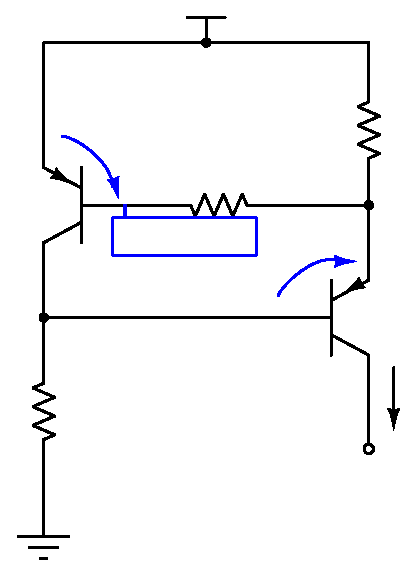
\includegraphics[scale=1]{fte}\\
   % translate x=384 y=372 scale 0.38
   \putbox{0.43in}{0.91in}{1.20}{$20 k\Omega$}%
   \putbox{2.56in}{2.83in}{1.20}{$100 \Omega$}%
   \putbox{1.47in}{2.54in}{1.20}{$2,2 k\Omega$}%
   \putbox{2.76in}{1.16in}{1.20}{$5 mA$}%
   \putbox{0.97in}{3.74in}{1.20}{VccH+}%
   \putbox{1.97in}{2.87in}{1.20}{R1}%
   \putbox{1.01in}{2.54in}{1.20}{R2}%
   \putbox{2.81in}{0.83in}{1.20}{$I_{pol}$}%
   \putbox{0.51in}{2.87in}{1.20}{$V_{BE}$}%
   \putbox{1.18in}{1.83in}{1.20}{$V_{BE}$}%
   \putbox{0.72in}{2.16in}{1.20}{\textcolor{blue}{$30V-V_{BE}$}}%
   } % close 'parbox'
   } % close 'scalebox'
   \vspace{-\baselineskip} % this is not necessary, but looks better
